% \begin{table*}[!t]
% \centering
% \scalebox{0.7}{
% \begin{tabular}{c|ccccc|c|ccc|c}
%     \toprule
%      & \multicolumn{5}{c|}{\textbf{Math Word Problems}} & \textbf{Planning} & \multicolumn{3}{c|}{\textbf{Multi-hop QA}} & \textbf{Logic} \\
%      \textbf{Method} & GSM8K & SVAMP & MultiArith & ASDiv & AQuA & SayCan & StrategyQA & Date & Sport  & CLUTRR \\
%      \hline
%      \multicolumn{11}{c}{Greedy Decoding} \vspace{0.05cm} \\
%      \hline
%      PAL/POT & 63.1 & 76.4 & 96.2 & 78.6 & 45.3 & 87.4 & \textbf{73.2} & 59.9 & 97.9 & 40.8 \\
%      Faithful CoT (ours)  & \textbf{72.1} & \textbf{83.5} & \textbf{98.8} & \textbf{80.0} & \textbf{47.2} & \textbf{90.3} & 63.0 & \textbf{80.8} & \underline{\textbf{99.1}} & \textbf{58.9} \\
%      \hline
%      \bottomrule

% \end{tabular}
% }
% \caption{Accuracy of different prompting methods on 10 reasoning datasets from 4 domains. We compare our method, Faithful CoT, with standard prompting \cite{brown_language_2020}, CoT prompting \cite{wei_chain_2022}, as well as previously published few-shot SOTA results. The best results within each decoding strategy are in \textbf{boldface}, and the new SOTA results across all strategies are \underline{underlined}.}
% \label{tab:main}
% \end{table*}

\begin{figure}
    \centering
    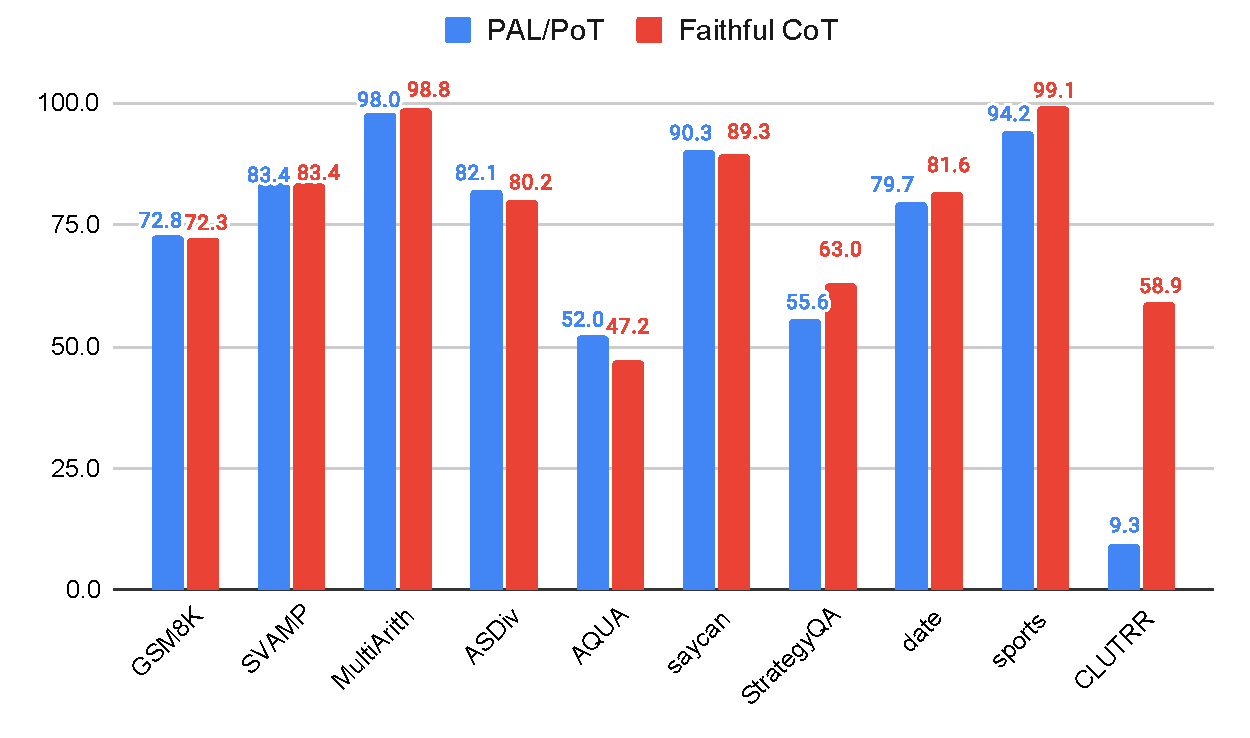
\includegraphics[width=\columnwidth]{img/fcot_vs_pal_pot.pdf}
    \caption{Accuracy of our method and two concurrent methods, Program of Thoughts (POT) \cite{chen_program_2022} and Program-Aided Language Models (PAL) \cite{gao_pal_2022}, on 10 reasoning datasets.}
    \label{fig:fcot_vs_pal_pot}
\end{figure}